\chapter{Sistema Andante}\label{chap:andante}

\section*{}

Neste capítulo é detalhado o sistema Andante, utilizado nos transportes públicos de passageiros da Área Metropolitana do Porto, permitindo contextualizar os conceitos e modalidades utilizados na aplicação.
\\O Andante é um título que permite viajar em diversos transportes públicos, de diferentes operadores, sendo o preço calculado baseado no trajeto a efetuar e não no modo de transporte utilizado ou o número de embarques realizados.
\\Os operadores aderentes ao sistema Andante são: Metro do Porto, STCP - Sociedade de Transportes Coletivos do Porto, CP - Comboios de Portugal, Resende, Espírito Santo, Maia Transportes, Valpi, Gondomarense, MGC Transportes, Nogueira da Costa e Auto-Viação Pacense. 

\section{Modalidades}

Os títulos Andante dividem-se em dois grandes grupos: Ocasionais e Assinaturas.

\subsection{Ocasionais}

Os títulos ocasionais estão disponíveis em duas alternativas: Título de Viagem e Andante 24. Tanto uma como outra utilizam o cartão azul, em papel, que não é personalizado e como tal permite a utilização por mais do que uma pessoa, desde que não seja em simultâneo.

\subsubsection{Título de Viagem}

Permite viajar durante um determinado período de tempo consoante o número de zonas compradas (Z2 – 2 anéis de zonas; Z3 – 3 anéis de zonas; e assim sucessivamente).
\\O mínimo de tempo que um título de viagem permite andar é de 1 hora. Este tempo de viagem aumenta à medida que cresce o número de zonas carregadas.

\subsubsection{Andante 24}

O funcionamento do Andante 24 é semelhante ao título de viagem, com a diferença de independentemente do número de zonas carregadas, permitir viajar durante as vinte e quatro horas seguintes à primeira validação.

\subsubsection{Andante Tour}

Título de transporte vocacionado para o segmento de turistas, confere acesso a toda a rede Andante permitindo um número ilimitado de viagens durante 24 horas (Andante Tour 1) ou 72 horas (Andante Tour 3) consecutivas após a primeira validação.
\\O cartão Andante Tour não é recarregável.


\subsection{Assinaturas}

As assinaturas permitem ao utilizador viajar dentro das zonas previamente selecionadas durante o período equivalente ao mês de calendário. Ao contrário dos títulos ocasionais, é necessário especificar quais as zonas pretendidas e a assinatura é apenas válida nessas zonas. O cartão da assinatura é o dourado, em plástico, e para além de fotografia inclui também o nome do utilizador, tornando-o de uso pessoal e intransmissível.
\\As assinaturas têm tarifas especiais para jovens, estudantes, reformados, pensionistas, seniores e beneficiários de ação social.

\section{Zonamento}

A rede de transportes públicos da Área Metropolitana do Porto está divida por zonas. Cada zona é constituída por uma letra e um número. As zonas estão agrupadas em três grandes grupos (Norte, Centro e Sul) e a inicial desse grupo serve para identificar a zona (N, C, S). Dentro de cada grupo as zonas são depois numeradas sequencialmente. Pode ver-se na Figura~\ref{fig:zonas} o zonamento Andante.
\\Este mapa é especialmente importante para perceber o número de zonas a carregar num título ocasional. Por exemplo, com um título Z2, entrando na zona C1 (centro do Porto), é possível viajar dentro dessa zona e em todas as que lhe sejam adjacentes (C2, C6 e S8). Por outro lado, usando um título Z3, pode viajar-se também até ao segundo anel de adjacência (C3, C5, C7, C8, C9, S1, S2, S7, S9). Ver Figura~\ref{fig:zonas_c1}.

\begin{figure}[t]
  \begin{center}
    \leavevmode
    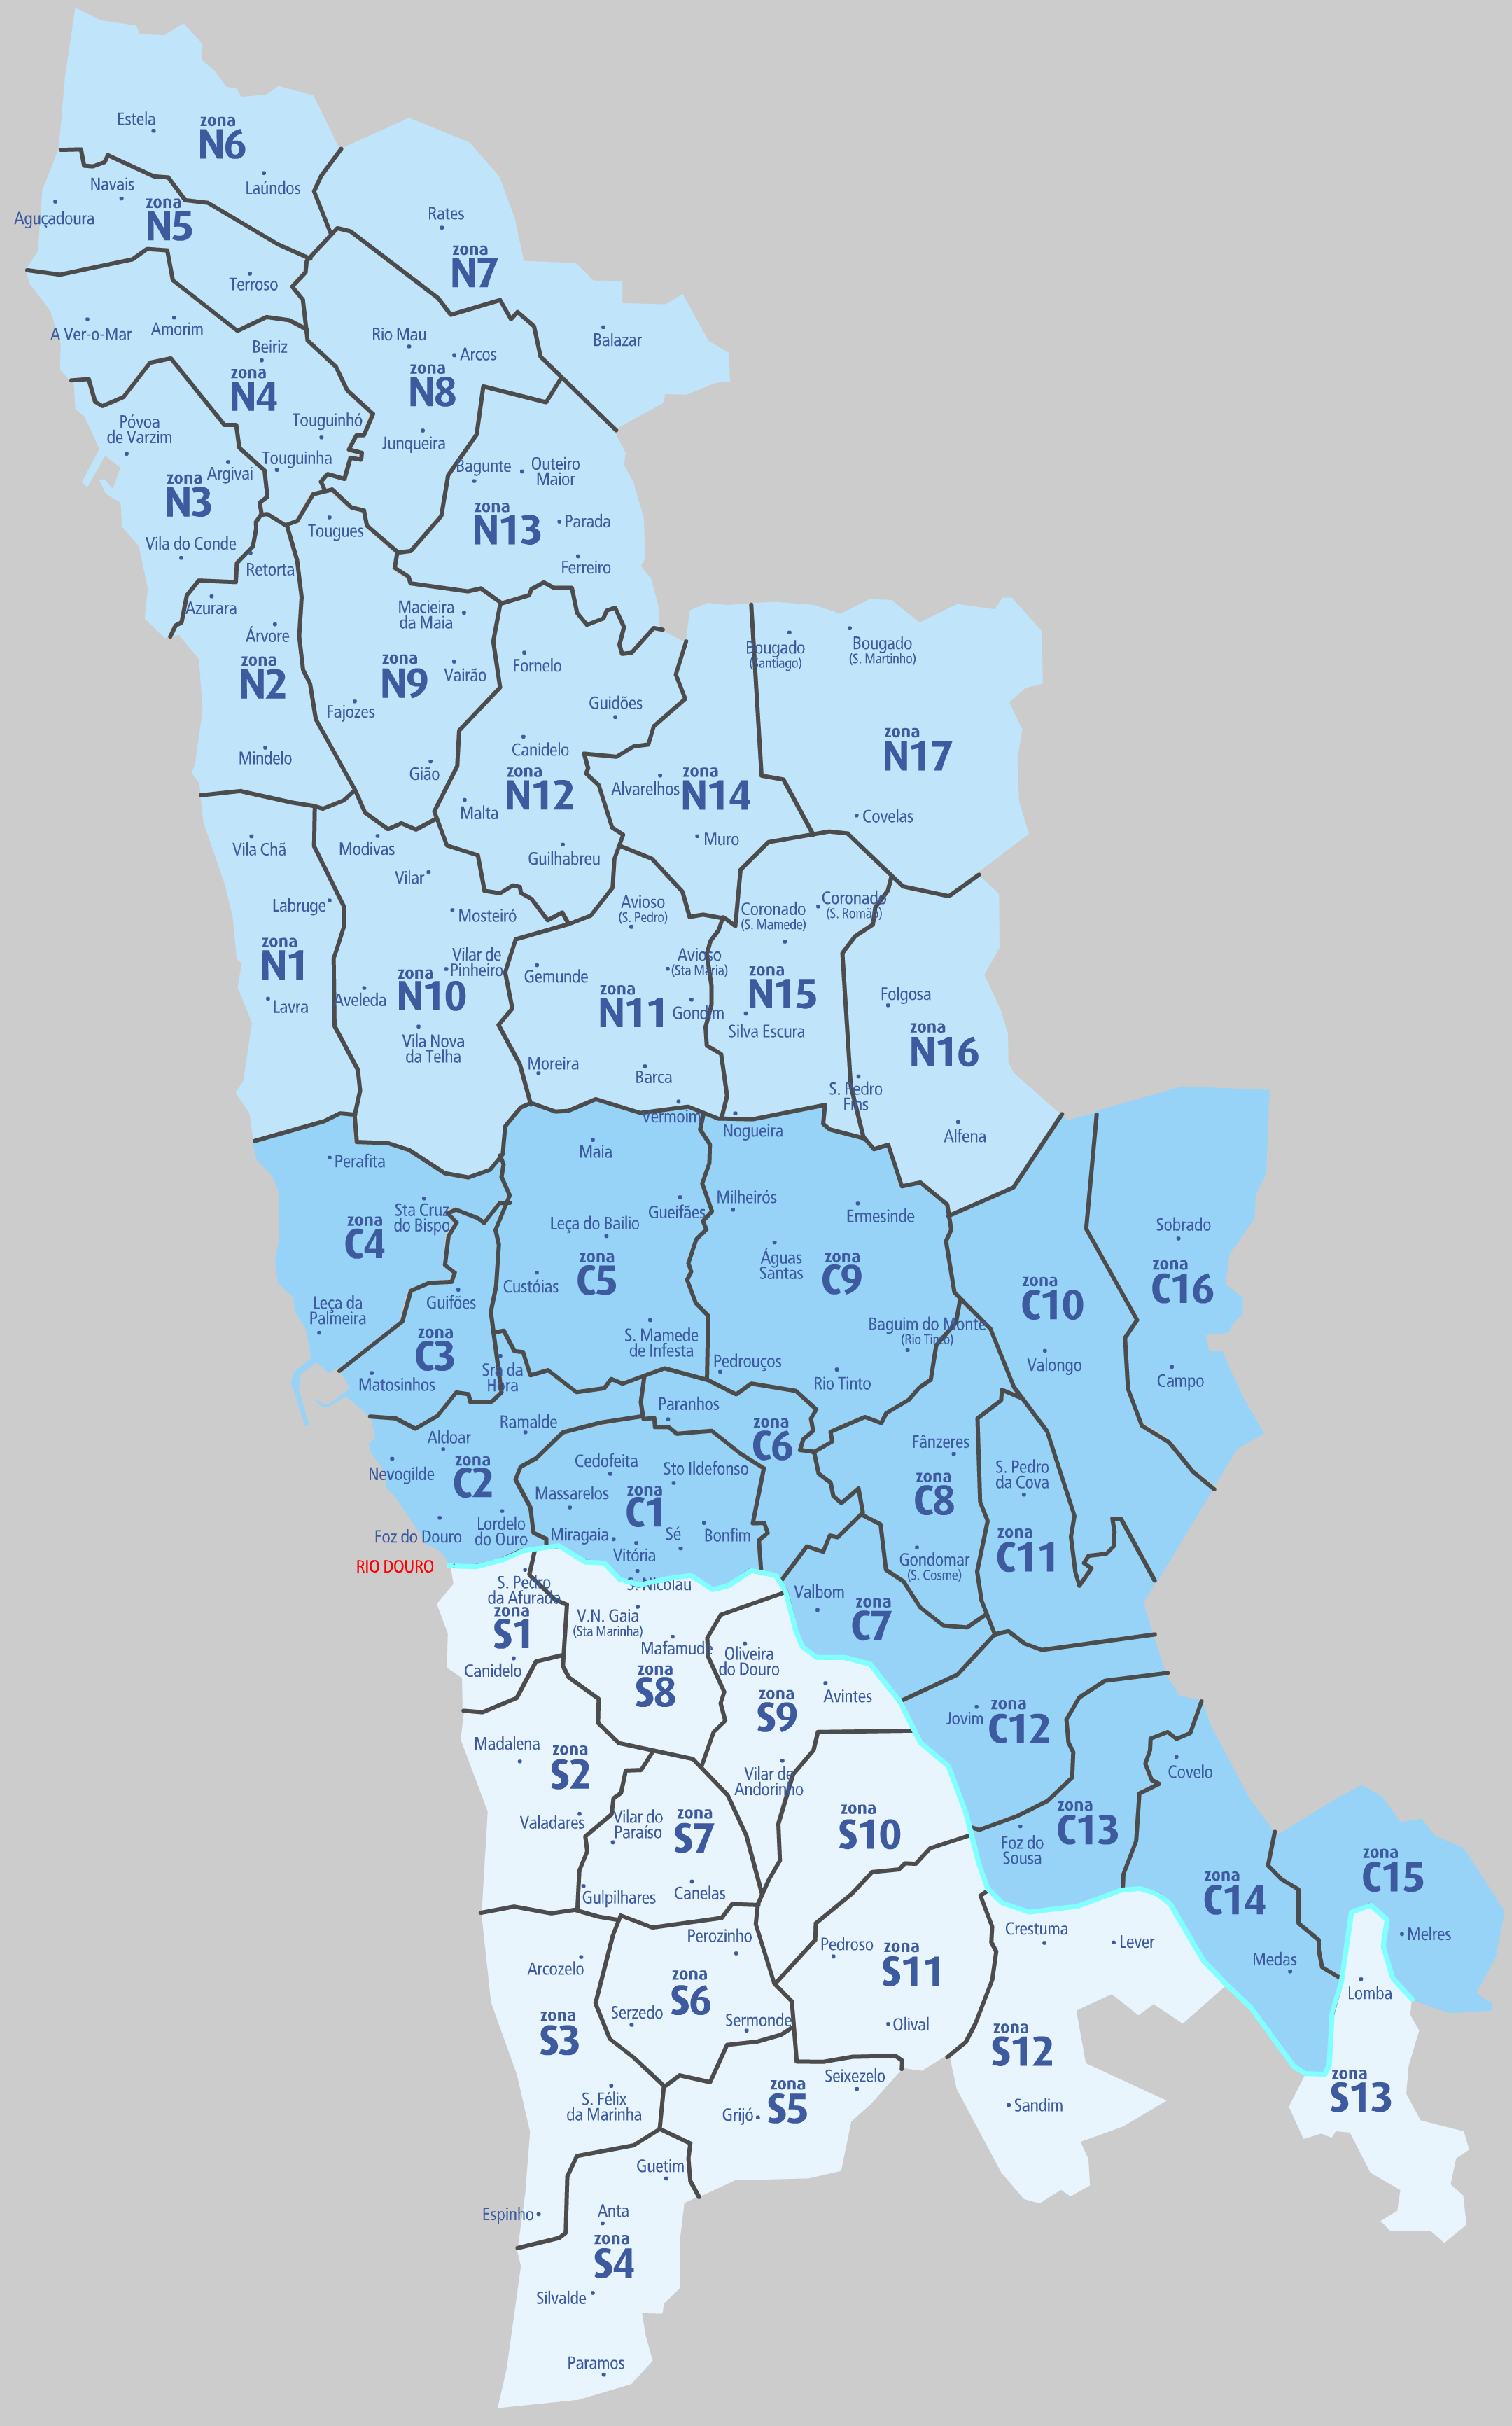
\includegraphics[scale=0.375]{zonas}
    \caption{Zonamento Andante}
    \label{fig:zonas}
  \end{center}
\end{figure}

\begin{figure}[t]
  \begin{center}
    \leavevmode
    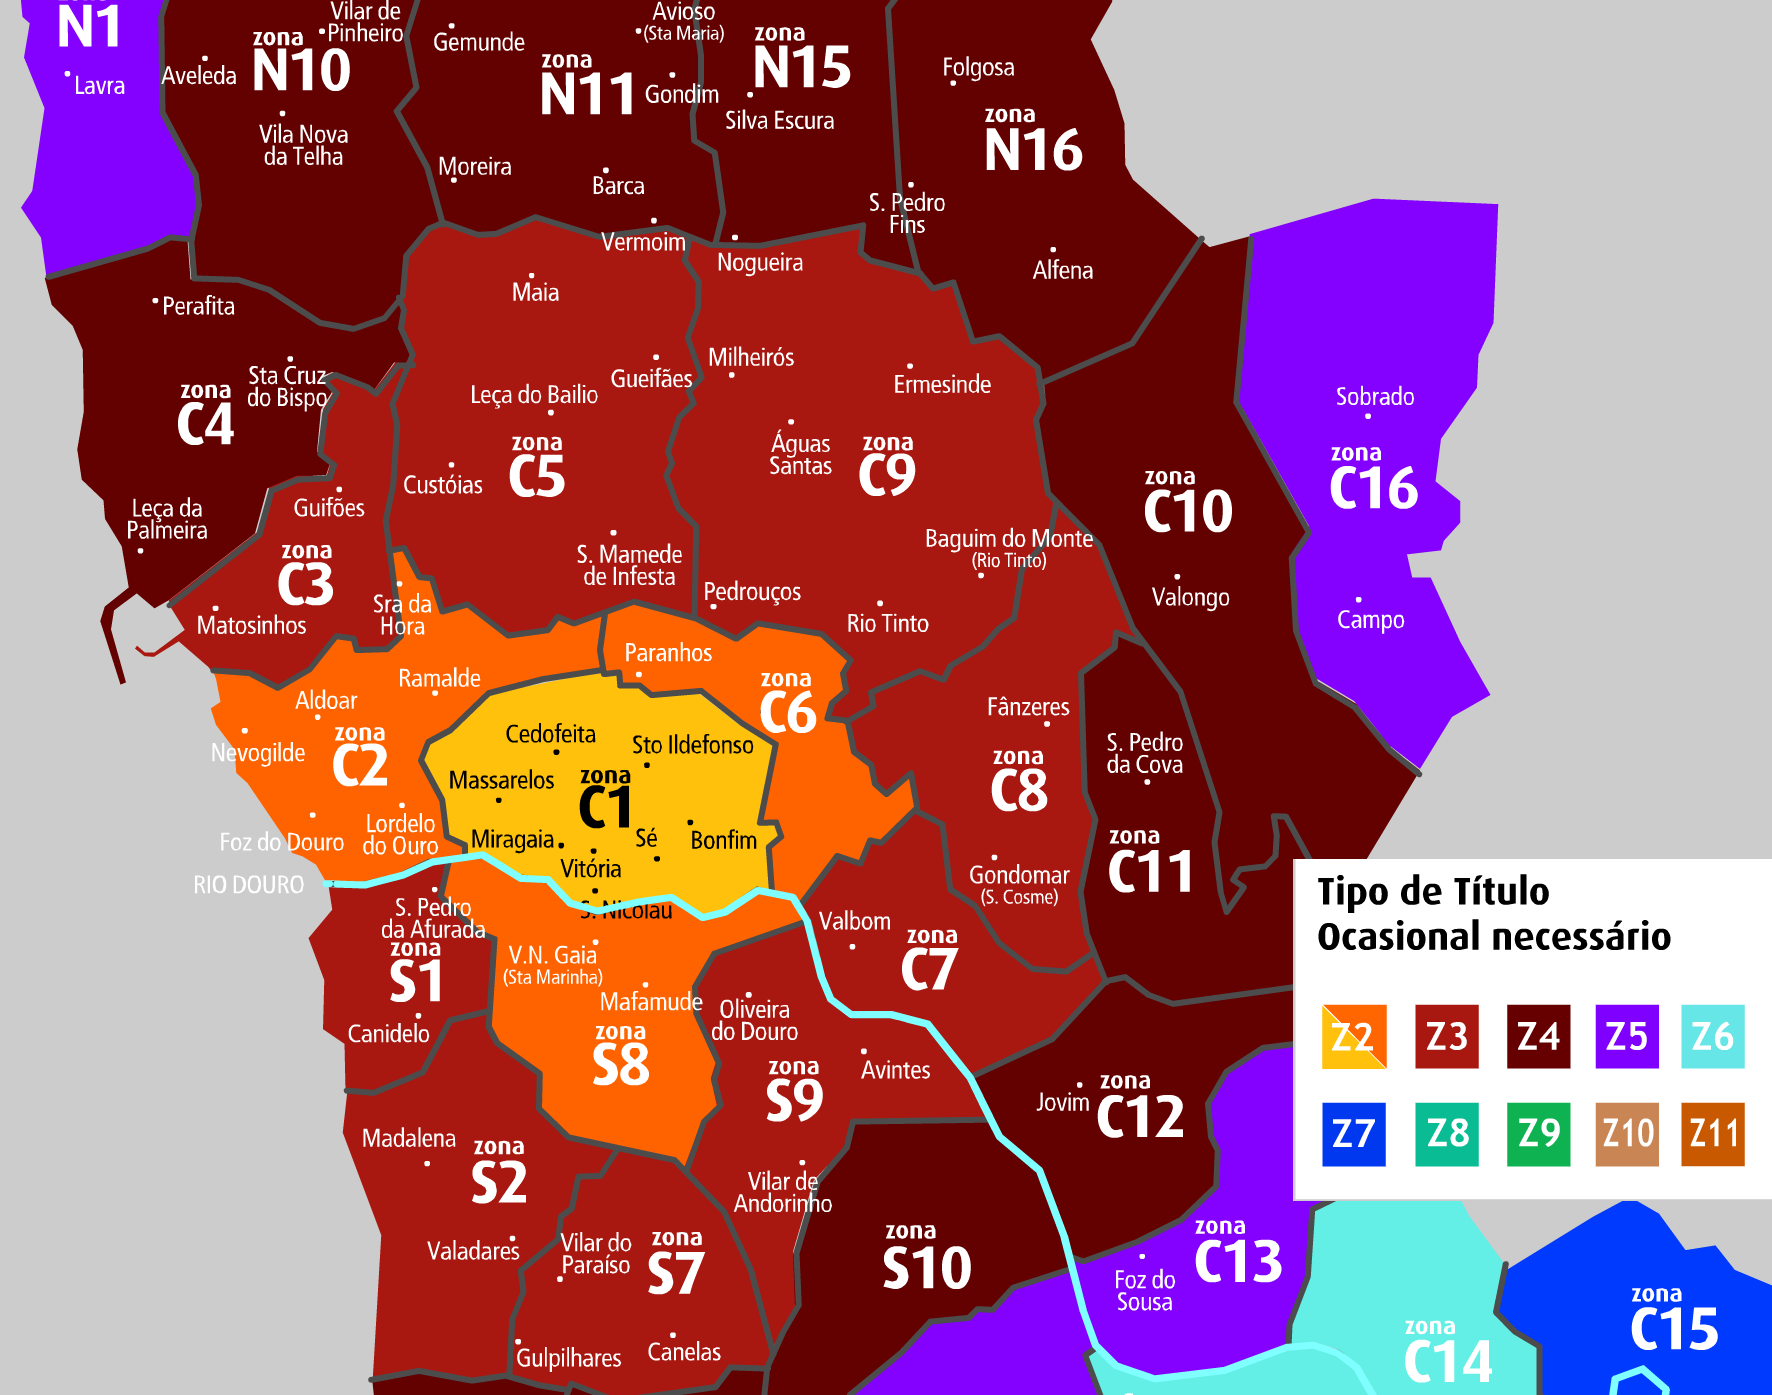
\includegraphics[scale=0.5]{zonas_c1}
    \caption{Cálculo de número de zonas Andante \cite{calczonas}}
    \label{fig:zonas_c1}
  \end{center}
\end{figure}

\section{Resumo ou Conclusões}

O sistema Andante traz aos transportes públicos da Área Metropolitana do Porto a comodidade e rapidez de utilizar apenas um só método de bilhética, permitindo aos operadores ter um sistema standard e familiar para o utilizador.
\\No entanto, muitas vezes os utilizadores ocasionais (turistas, por exemplo) têm alguma dificuldade em perceber o funcionamento do sistema Andante devido à sua complexidade, nomeadamente ao cálculo de zonas necessárias para efetuar determinada viagem. Sendo que uma viagem poderá necessitar de número de zonas diferentes consoante o sentido em que é feito, devido ao facto de os percursos de ida e volta nem sempre coincidirem.